\documentclass[11pt]{article}

% Change "review" to "final" to generate the final (sometimes called camera-ready) version.
% Change to "preprint" to generate a non-anonymous version with page numbers.
\usepackage[review]{acl}

% Standard package includes
\usepackage{times}
\usepackage{latexsym}
\usepackage{multirow}
\usepackage{arydshln}
\setlength{\dashlinedash}{0.5pt}
\setlength{\dashlinegap}{1.5pt}
\usepackage{amsmath}
\usepackage[most]{tcolorbox}

\usepackage{graphicx}
\usepackage{amsmath}
\usepackage{amssymb}
\usepackage{svg}

\usepackage{booktabs}   % \toprule, \midrule, \bottomrule, \cmidrule
\usepackage{graphicx}   % \resizebox (only if the table overflows)


% For proper rendering and hyphenation of words containing Latin characters (including in bib files)
\usepackage[T1]{fontenc}
% For Vietnamese characters
% \usepackage[T5]{fontenc}
% See https://www.latex-project.org/help/documentation/encguide.pdf for other character sets

% This assumes your files are encoded as UTF8
\usepackage[utf8]{inputenc}

% This is not strictly necessary, and may be commented out,
% but it will improve the layout of the manuscript,
% and will typically save some space.
\usepackage{microtype}

% This is also not strictly necessary, and may be commented out.
% However, it will improve the aesthetics of text in
% the typewriter font.
\usepackage{inconsolata}

%Including images in your LaTeX document requires adding
%additional package(s)
\usepackage{graphicx}

% If the title and author information does not fit in the area allocated, uncomment the following
%
%\setlength\titlebox{<dim>}
%
% and set <dim> to something 5cm or larger.

\title{A Graph-Based Approach to Analyzing Human-LLM Reasoning paths in Scientific Fact-Checking}

% Author information can be set in various styles:
% For several authors from the same institution:
% \author{Author 1 \and ... \and Author n \\
%         Address line \\ ... \\ Address line}
% if the names do not fit well on one line use
%         Author 1 \\ {\bf Author 2} \\ ... \\ {\bf Author n} \\
% For authors from different institutions:
% \author{Author 1 \\ Address line \\  ... \\ Address line
%         \And  ... \And
%         Author n \\ Address line \\ ... \\ Address line}
% To start a separate ``row'' of authors use \AND, as in
% \author{Author 1 \\ Address line \\  ... \\ Address line
%         \AND
%         Author 2 \\ Address line \\ ... \\ Address line \And
%         Author 3 \\ Address line \\ ... \\ Address line}

\author{First Author \\
  Affiliation / Address line 1 \\
  Affiliation / Address line 2 \\
  Affiliation / Address line 3 \\
  \texttt{email@domain} \\\And
  Second Author \\
  Affiliation / Address line 1 \\
  Affiliation / Address line 2 \\
  Affiliation / Address line 3 \\
  \texttt{email@domain} \\}

%\author{
%  \textbf{First Author\textsuperscript{1}},
%  \textbf{Second Author\textsuperscript{1,2}},
%  \textbf{Third T. Author\textsuperscript{1}},
%  \textbf{Fourth Author\textsuperscript{1}},
%\\
%  \textbf{Fifth Author\textsuperscript{1,2}},
%  \textbf{Sixth Author\textsuperscript{1}},
%  \textbf{Seventh Author\textsuperscript{1}},
%  \textbf{Eighth Author \textsuperscript{1,2,3,4}},
%\\
%  \textbf{Ninth Author\textsuperscript{1}},
%  \textbf{Tenth Author\textsuperscript{1}},
%  \textbf{Eleventh E. Author\textsuperscript{1,2,3,4,5}},
%  \textbf{Twelfth Author\textsuperscript{1}},
%\\
%  \textbf{Thirteenth Author\textsuperscript{3}},
%  \textbf{Fourteenth F. Author\textsuperscript{2,4}},
%  \textbf{Fifteenth Author\textsuperscript{1}},
%  \textbf{Sixteenth Author\textsuperscript{1}},
%\\
%  \textbf{Seventeenth S. Author\textsuperscript{4,5}},
%  \textbf{Eighteenth Author\textsuperscript{3,4}},
%  \textbf{Nineteenth N. Author\textsuperscript{2,5}},
%  \textbf{Twentieth Author\textsuperscript{1}}
%\\
%\\
%  \textsuperscript{1}Affiliation 1,
%  \textsuperscript{2}Affiliation 2,
%  \textsuperscript{3}Affiliation 3,
%  \textsuperscript{4}Affiliation 4,
%  \textsuperscript{5}Affiliation 5
%\\
%  \small{
%    \textbf{Correspondence:} \href{mailto:email@domain}{email@domain}
%  }
%}

\begin{document}
\maketitle
\begin{abstract}

\end{abstract}

\section{Introduction}



\paragraph{Research Questions.}
Research questions:

\begin{itemize}
    \item Given a misleading scientific claim and its cited study as evidence, how reliably do LLMs predict \textit{Incorrect} verdict across repeated seeds?

    \item  To what extent do LLM reasoning paths align with the reasoning paths used by human experts?

    \item  For LLM reasoning paths that diverge from human reasoning, are they grounded in the cited study and logically sound?
\end{itemize}

\section{Related Work}

Scientific fact-checking has commonly been framed as verifying claims against scientific or biomedical evidence. Benchmarks such as SciFact evaluate evidence retrieval, rationale selection, and veracity prediction for scientific claims \citep{wadden-etal-2020-fact}. Related health and biomedical datasets, including PUBHEALTH, HEALTHVER, and HealthFC, similarly focus on checking public-health or biomedical claims against evidence and assigning veracity labels \citep{kotonya-toni-2020-explainable-automated,sarrouti-etal-2021-evidence-based,vladika-etal-2024-healthfc}. Later work extends this setting to open-domain and richer evidence scenarios, such as SciFact-Open, SciVer, and long-document claim--evidence linking in CLAIM-BENCH \citep{wadden-etal-2022-scifact,wang-etal-2025-sciver,javaji-etal-2025-ai}. These studies establish the importance of grounding verdicts in scientific evidence, but they mainly evaluate final labels, retrieved evidence, or rationale selection. They do not ask whether a model that predicts the correct verdict follows the same reasoning path as a human expert when both are given the same misleading claim and cited study.

A closely related line of work studies the misrepresentation of scientific evidence. MISSCI models misleading scientific claims as fallacious arguments, where a real study is used to support an inaccurate claim through an implicit but invalid reasoning step \citep{glockner-etal-2024-missci}. MISSCIPLUS extends this setting by grounding such fallacies in real passages from the misrepresented scientific publications \citep{glockner-etal-2025-grounding}. These works are especially relevant because they move scientific fact-checking beyond surface-level verdict prediction and show that misinformation often arises from distorted reasoning over otherwise valid evidence. However, their main objective is to reconstruct missing fallacious premises, ground them in study passages, or classify fallacy types. They do not compare human expert explanations and LLM explanations as parallel reasoning structures, nor do they evaluate whether an LLM uses the same study context, study findings, fallacy-supporting premise, and fallacy label as the human expert.

Recent work has also evaluated LLMs for fact-checking and biomedical claim verification. Studies on zero-shot scientific claim verification, structured biomedical prompting, step-by-step medical verification, and explainable public-health fact-checking show that LLMs can generate plausible verdicts and explanations when guided by evidence or structured prompts \citep{alvarez2024zero,liang2025advancing,vladika2025step,zarharan2024tell,tan2025improving}. However, work on explanation faithfulness shows that model-generated explanations may appear plausible without faithfully reflecting the underlying decision process \citep{turpin2023language,atanasova2023faithfulness,parcalabescu2024measuring}. This motivates our focus on reasoning-path alignment: a correct verdict and fluent explanation do not necessarily show that the model interpreted the cited study in the same way as an expert fact-checker.

Our work is also related to human rationale and structured explanation research. Datasets such as e-SNLI and ERASER introduced human explanations and rationales as evaluation targets beyond final labels \citep{camburu2018esnli,deyoung2020eraser}. Work on explanation graphs and multi-step reasoning, such as WorldTree and EntailmentBank, represents explanations as connected reasoning structures rather than unstructured text \citep{jansen2018worldtree,xie2020worldtree,dalvi2021explaining}. Argument-mining research similarly models claims, premises, warrants, and support relations in argumentative text \citep{lawrence2019argument}. Building on these ideas, our study represents each fact-checking explanation as a structured reasoning graph connecting the claim, study context, study findings, fallacy-supporting premises, and fallacies. This allows us to compare human and LLM reasoning at the fallacy-entry level rather than only through whole-explanation similarity or evidence-span overlap.

Finally, our analysis connects to grounding and hallucination evaluation. Prior work on attribution, citation faithfulness, QA-based factuality checking, and atomic-fact evaluation examines whether generated statements are supported by source documents \citep{gao2023enabling,min2023factscore,fabbri2022qafacteval,tang2024minicheck,li2024attributionbench}. These approaches are useful for detecting unsupported content, but they usually evaluate grounding at the level of claims, answer sentences, citations, or atomic facts. Our study shifts the focus from grounded statements to grounded reasoning paths. For LLM graphs that do not align with human graphs, we further examine whether the alternative reasoning is still supported by the cited study and logically valid, distinguishing aligned expert-like reasoning from valid but different reasoning, hallucination, and logically unsound reasoning.

Overall, prior work has studied scientific claim verification, fallacy reconstruction, explainable fact-checking, rationale alignment, structured explanation, and grounding evaluation. However, these lines of work have largely remained separate. Our study addresses this gap by asking whether LLMs that correctly identify misleading scientific claims as incorrect reach that verdict through the same evidence-to-fallacy reasoning path as human experts. By representing explanations as structured reasoning graphs, aligning them at the fallacy-entry level, and analyzing non-aligned reasoning for grounding and logical soundness, our work moves beyond verdict accuracy toward a process-level evaluation of human--LLM reasoning alignment in scientific fact-checking.

\section{Graph-Based Analysis of Human--LLM Reasoning}
\label{sec:reasoning-graph-method}

We investigate whether LLMs follow the same reasoning path as human experts when both are given the same incorrect claim and the same cited scientific study. 
Beyond verdict accuracy, we compare the reasoning structures used by humans and LLMs in terms of study context, study findings, fallacy-supporting premises, and fallacy labels. 
When an LLM reasoning graph does not align with the corresponding human graph, we further assess whether the LLM's alternative reasoning path is grounded in the cited study and logically sound.

Each instance contains an incorrect or misleading claim paired with its cited study. 
Since all input claims are incorrect, the expected verdict is \textit{Incorrect}. 
We therefore focus the reasoning-graph analysis on LLM outputs with an \textit{Incorrect} verdict, as these verdicts are label-consistent and can be compared with the human expert reasoning for the same claim--study pair.

Figure~\ref{fig:methodology} summarizes the workflow. 
We first compute LLM verdict distributions across repeated runs. 
We then convert selected \textit{Incorrect}-verdict explanations into reasoning graphs, compare them with human graphs, and validate non-aligned LLM graphs for grounding and logical soundness.

\begin{figure*}[t]
    \centering
    
\includegraphics[width=\textwidth]{latex/approach.png}
    \caption{Graph-based analysis of human--LLM reasoning. For \textit{Incorrect}-verdict cases, human and LLM explanations are converted into reasoning graphs and compared for alignment. Non-aligned LLM graphs are further validated for study grounding and logical soundness.}
    \label{fig:methodology}
\end{figure*}

\subsection{LLM Verdict Computation}
\label{subsec:verdict-computation}

For each claim--study pair, the LLM produces one of four verdicts: 
\textit{Correct}, \textit{Incorrect}, \textit{Not Enough Information (NEI)}, or \textit{No Response}. 
\textit{No Response} is assigned when the model output does not contain a valid verdict.

For each experimental configuration, defined by the model, prompt, and evidence type, we run the same input three times to account for output variability. 
For claim $i$ and verdict label $\ell$, we compute the per-claim proportion:

\begin{equation}
p_{i,\ell} = \frac{n_{i,\ell}}{3},
\end{equation}

\noindent
where $n_{i,\ell}$ is the number of times label $\ell$ appears across the three runs. 
We then average these proportions over all $N$ claims:

\begin{equation}
\bar{p}_{\ell} = \frac{1}{N} \sum_{i=1}^{N} p_{i,\ell} \times 100 .
\end{equation}

\noindent
The resulting $\bar{p}_{\ell}$ gives the percentage distribution of each verdict label. 
We also report consistency as the proportion of claims for which all three runs produce the same verdict.

\subsection{Reasoning Graph Representation}
\label{subsec:reasoning-graph}

For reasoning-graph analysis, we select only \textit{Incorrect}-verdict explanations, where the LLM verdict aligns with the expected human verdict, and represent both human and LLM explanations using the same reasoning-graph schema:

\begin{quote}
\small
\textit{Claim} $\rightarrow$ \textit{Study Context} $\rightarrow$ \textit{Study Findings} $\rightarrow$ \textit{Fallacy-Supporting Premises} $\rightarrow$ \textit{Fallacies}.
\end{quote}

\noindent
\textit{Study Context} captures the study design, population, scope, or experimental setting. 
\textit{Study Findings} captures the relevant results or conclusions reported in the cited study. 
\textit{Fallacy-Supporting Premises} identify how the claim misrepresents the study and why a particular fallacy label applies. 
\textit{Fallacies} denote the reasoning errors assigned to the claim.

Formally, each graph is represented as $G=(V,E)$, where $V$ is the set of reasoning components and $E$ denotes directed reasoning relations among them. 
We treat the human reasoning graph as the reference graph and compare it with the corresponding LLM graph for the same claim--study pair.

\subsection{Human--LLM Reasoning Graph Alignment}
\label{subsec:graph-alignment}

An LLM reasoning graph may contain one or more fallacy entries. 
We therefore evaluate alignment at the level of individual fallacy entries. 
Each entry consists of four components: study context, study findings, fallacy-supporting premise, and fallacy type.

For each LLM fallacy entry $f_i^{L}$, we identify human fallacy entries for the same claim--study pair with the same fallacy type. 
If no same-type human entry exists, the LLM entry is marked as unmatched. 
If exactly one exists, the two entries are paired. 
If multiple same-type human entries exist, we pair the LLM entry with the human entry whose fallacy-supporting premise has the highest cosine similarity. 
Cosine similarity is used only for candidate selection, not for the final match decision.

For a paired LLM--human fallacy entry $(f_i^{L}, f_j^{H})$, we define a binary match variable $m_i$:

\begin{equation}
\begin{aligned}
m_i =
\mathbb{I}\big[
&\mathrm{type}(f_i^{L}) = \mathrm{type}(f_j^{H}) \\
&\land\; \forall c \in \mathcal{C},\;
\mathrm{STS}_c(f_i^{L}, f_j^{H}) \geq 3
\big].
\end{aligned}
\end{equation}

\noindent
Here, $\mathcal{C}$ contains the three textual components: study context, study findings, and fallacy-supporting premise. 
The indicator function $\mathbb{I}[\cdot]$ returns 1 only when the paired entries have the same fallacy type and each textual component has an STS score of at least 3. 
We use $\mathrm{STS}\geq3$ because it is the lowest score indicating that two texts describe the same semantic facet, even if some details differ.

At the graph level, an LLM reasoning graph is considered aligned with the human reference graph if at least one of its fallacy entries satisfies the fallacy-level match criterion:

\begin{equation}
M_G =
\mathbb{I}\left[
\exists i \in \mathcal{F}_{G}^{L} : m_i = 1
\right],
\end{equation}

\noindent
where $M_G$ denotes whether the LLM graph $G$ is aligned with the corresponding human graph, and $\mathcal{F}_{G}^{L}$ denotes the set of fallacy entries in the LLM graph. 
Thus, graph-level alignment requires that the LLM produce at least one reasoning path that is semantically and structurally aligned with the human expert graph.

\subsection{Validation of Non-Aligned LLM Graphs}
\label{subsec:validation}

If the LLM graph does not align with the human graph, we do not automatically treat it as invalid. 
A non-aligned graph may still represent a different but valid reasoning path if it is grounded in the cited study and logically sound. 
We therefore validate non-aligned LLM graphs using grounding and logical-soundness checks.

\subsubsection{Grounding Validation}
\label{subsubsec:grounding}

We first check whether the LLM graph components are grounded in the cited study. 
The QA-based grounding check verifies whether the study context, study findings, and fallacy-supporting premises are supported by the study text. 
If the QA-based check marks a component as ungrounded, we perform a human re-check to verify the grounding decision, since the QA method may incorrectly reject a grounded component.

If the component remains unsupported after human re-check, the case is classified as hallucination. 
We define hallucination as a reasoning component asserted by the LLM that is not supported by the cited study.

\subsubsection{Logical Soundness Validation}
\label{subsubsec:logical-soundness}

For grounded LLM graphs, we further assess whether the reasoning is logically sound. 
A graph is considered logically sound when the fallacy-supporting premises correctly connect the claim, the cited study evidence, and the assigned fallacy label. 
It is considered logically unsound when the evidence is grounded but the inference is invalid, such as applying the wrong fallacy type, overextending the study findings, or drawing an unsupported conclusion.

\subsection{Outcome Categories}
\label{subsec:outcome-categories}

Each selected \textit{Incorrect}-verdict case is assigned to one of four categories:

\paragraph{Aligned reasoning.}
The LLM graph aligns with the human reference graph.

\paragraph{Valid but different reasoning path.}
The LLM graph does not align with the human graph, but it is grounded in the cited study and logically sound.

\paragraph{Hallucination.}
The LLM graph contains a reasoning component that is not supported by the cited study, even after human re-check.

\paragraph{Logically unsound reasoning.}
The LLM graph is grounded in the cited study, but the reasoning from evidence to fallacy label is not logically valid.




\section{Experimetns}

\paragraph{Veracity Computation}
Table~\ref{tab:combined_results} presents the distribution of model predictions
in a claim verification task. For each claim, a model outputs one verdict:
\textit{Correct}, \textit{Incorrect}, \textit{Not Enough Information (NEI)}, or \textit{No Response}.
The \textit{No Response} label is assigned when the model does not return a valid verdict.

For each configuration (model, prompt, and evidence type), the same input is evaluated
three times, producing three verdicts per claim. We compute veracity in two steps:

\textbf{Step 1: Per-claim proportions.}
For each claim, we run the same input prompt three times and record the verdict produced in each run.
For example, if the model predicts \textit{Incorrect} in two runs and \textit{Correct} in one run,
then \textit{NEI} and \textit{No Response} receive a value of $0$ because they were not produced for this claim.
The per-claim veracity proportions are therefore: Incorrect = $2/3$, Correct = $1/3$, NEI = $0$, and No Response = $0$.

We apply this procedure to all claims in the experimental setting. The final value for each verdict label is then computed by averaging its per-claim proportions across all claims.  

\textbf{Step 2: Aggregation across claims.}
We then average these proportions over all $N$ claims:
\[
\bar{p}_{\ell} = \frac{1}{N} \sum_{i=1}^{N} \frac{n_{i,\ell}}{3} \times 100,
\]
where $n_{i,\ell}$ denotes the number of times label $\ell$ appears
among the three runs for claim $i$.

The resulting values $\bar{p}_{\ell}$ represent the final distribution of verdict labels
reported in Table~\ref{tab:combined_results}.

We also measure \emph{consistency} as the proportion of claims for which all three
runs produce the same verdict.


Table~\ref{tab:combined_results} presents the performance of LLMs as fact-checkers, where each model is given a claim and its associated scientific evidence and predicts a final verdict: \textit{Correct}, \textit{Incorrect}, \textit{Not Enough Information (NEI)}, or \textit{No Response}. 
We evaluate two prompting strategies—a \textit{Short} prompt from MISSCIPlus and our \textit{Detailed} prompt—and two evidence settings: \textit{Selected Passages} and \textit{Full Study}. 
For each configuration, the model is run three times with the same inputs. Each run produces one veracity label per claim.

For each label $l$ in run $r$, we compute its percentage as:
\[
P_r(l)=\frac{N_r(l)}{N}\times 100,
\]
where $N_r(l)$ is the number of claims assigned label $l$ in run $r$, and $N$ is the total number of claims. 
The final reported value is the average percentage across the three runs:
\[
P(l)=\frac{1}{3}\sum_{r=1}^{3}P_r(l).
\]

In addition, we measure model \emph{consistency}, defined as the proportion of claims for which all three runs produce the same verdict. The table reports the resulting average distribution of veracity labels together with consistency scores.



\begin{table*}[t]
\centering
\small
\setlength{\tabcolsep}{4pt}
\begin{tabular}{ll l cccc c}
\hline
\textbf{Model} & \textbf{Evidence} & \textbf{Prompt} & \textbf{Correct} & \textbf{Incorrect} & \textbf{NEI} & \textbf{No Response} & \textbf{Consistency} \\
\hline

\multirow{4}{*}{\textbf{Qwen3-32B}} 
& \multirow{2}{*}{Full Study} 
& Short Prompt    & 30.56 & 39.68 & 29.76 & 0.00 & 80.95 \\
& 
& Detailed Prompt & 23.81 & 73.41 & 2.78  & 0.00 & 85.71 \\
& \multirow{2}{*}{Selected Passages} 
& Short Prompt    & 27.78 & 31.75 & 40.48 & 0.00 & 79.76 \\
& 
& Detailed Prompt & 19.84 & \underline{\textbf{76.98}} & 3.17  & 0.00 & \underline{86.90} \\
\hline

\multirow{4}{*}{\textbf{GPT-5}} 
& \multirow{2}{*}{Full Study} 
& Short Prompt    & 20.63 & 32.54 & 46.83 & 0.00 & 71.43 \\
& 
& Detailed Prompt & 15.87 & \underline{74.60} & 9.52  & 0.00 & 72.62 \\
& \multirow{2}{*}{Selected Passages} 
& Short Prompt    & 18.65 & 42.46 & 38.10 & 0.79 & 77.38 \\
& 
& Detailed Prompt & 19.05 & 69.05 & 11.90 & 0.00 & \underline{95.24} \\
\hline

\multirow{4}{*}{\textbf{Claude Opus 4.7}} 
& \multirow{2}{*}{Full Study} 
& Short Prompt    & 32.14 & 19.84 & 45.63 & 2.38 & 87.80 \\
& 
& Detailed Prompt & 38.55 & \underline{44.58} & 15.66 & 1.20 & \underline{\textbf{100.00}} \\
& \multirow{2}{*}{Selected Passages} 
& Short Prompt    & 48.81 & 34.52 & 16.67 & 0.00 & 95.24 \\
& 
& Detailed Prompt & 33.33 & 38.10 & 26.19 & 2.38 & \underline{\textbf{100.00}} \\
\hline

\end{tabular}
\caption{LLM-based fact-checking performance across prompting strategies and evidence settings.
Values report average verdict distribution (\%) over three runs and model consistency (agreement across runs).
Underlined values indicate the best per model, and \textbf{bold} the best overall.}

\label{tab:combined_results}
\end{table*}

\begin{table}[t]
\centering
\caption{Fallacy-set agreement between human and LLM reasoning graphs. Precision, Recall, and F1 are micro-averaged. Claude and Qwen results are placeholders.}
\label{tab:fallacy_eval}
\scriptsize
\setlength{\tabcolsep}{2pt}
\resizebox{\columnwidth}{!}{%
\begin{tabular}{@{}lcccccc@{}}
\toprule
\textbf{LLM} 
& \textbf{Exact} 
& \textbf{At-Least} 
& \textbf{Jaccard} 
& \textbf{Precision} 
& \textbf{Recall} 
& \textbf{F1} \\
& \textbf{Match}
& \textbf{One Match}
& \textbf{Similarity}
& 
& 
& \\
\midrule
GPT-5  & 0.167 & 0.500 & 0.323 & 0.398 & 0.413 & 0.405 \\
Claude & 0.000 & 0.000 & 0.000 & 0.000 & 0.000 & 0.000 \\
Qwen   & 0.000 & 0.000 & 0.000 & 0.000 & 0.000 & 0.000 \\
\bottomrule
\end{tabular}%
}
\end{table}




\begin{table*}[t]
\centering
\caption{Component-level analysis of human vs LLM reasoning graphs:
STS rubric score distributions from three judge LLMs (Model column), with
$\alpha$ as Krippendorff's ordinal inter-judge agreement. Cells are placeholders pending runs.}
\label{tab:sts_distribution}
\footnotesize
\setlength{\tabcolsep}{4pt}
\resizebox{\textwidth}{!}{%
\begin{tabular}{@{}ll*{6}{c}*{6}{c}*{6}{c}*{6}{c}c@{}}
\toprule
& & \multicolumn{6}{c}{\textbf{StudyContext}}
& \multicolumn{6}{c}{\textbf{StudyResult}}
& \multicolumn{6}{c}{\textbf{AddPremises h$\to$llm}}
& \multicolumn{6}{c}{\textbf{AddPremises llm$\to$h}}
& \\
\cmidrule(lr){3-8} \cmidrule(lr){9-14} \cmidrule(lr){15-20} \cmidrule(lr){21-26}
\textbf{Graphs} & \textbf{Judges}
 & 5 & 4 & 3 & 2 & 1 & 0
 & 5 & 4 & 3 & 2 & 1 & 0
 & 5 & 4 & 3 & 2 & 1 & 0
 & 5 & 4 & 3 & 2 & 1 & 0
 & \textbf{$\alpha$} \\
\midrule
\multirow{3}{*}{Human vs GPT-5}
 & GPT-5  & 0 & 35 & 11 & 18 & 2 & 0 & 2 & 44 & 20 & 16 & 1 & 1 & 3 & 53 & 30 & 73 & 17 & 6 & 3 & 49 & 26 & 76 & 13 & 4 & \multirow{3}{*}{0.778} \\
 & Claude Opus 4.7 & 1 & 34 & 16 & 6 & 0 & 1 & 6 & 34 & 17 & 15 & 4 & 1 & 4 & 31 & 38 & 52 & 36 & 16 & 6 & 30 & 42 & 43 & 32 & 11 & \\
 & Qwen3-32B   & 0 & 38 & 3 & 23 & 1 & 1 & 0 & 42 & 22 & 19 & 0 & 1 & 0 & 34 & 21 & 97 & 24 & 6 & 2 & 32 & 21 & 96 & 18 & 2 & \\
\midrule
\multirow{3}{*}{Human vs Claude}
 & GPT-5  & 0 & 0 & 0 & 0 & 0 & 0 & 0 & 0 & 0 & 0 & 0 & 0 & 0 & 0 & 0 & 0 & 0 & 0 & 0 & 0 & 0 & 0 & 0 & 0 & \multirow{3}{*}{0.000} \\
 & Claude Opus 4.7 & 0 & 0 & 0 & 0 & 0 & 0 & 0 & 0 & 0 & 0 & 0 & 0 & 0 & 0 & 0 & 0 & 0 & 0 & 0 & 0 & 0 & 0 & 0 & 0 & \\
 & Qwen3-32B   & 0 & 0 & 0 & 0 & 0 & 0 & 0 & 0 & 0 & 0 & 0 & 0 & 0 & 0 & 0 & 0 & 0 & 0 & 0 & 0 & 0 & 0 & 0 & 0 & \\
\midrule
\multirow{3}{*}{Human vs Qwen}
 & GPT-5  & 0 & 0 & 0 & 0 & 0 & 0 & 0 & 0 & 0 & 0 & 0 & 0 & 0 & 0 & 0 & 0 & 0 & 0 & 0 & 0 & 0 & 0 & 0 & 0 & \multirow{3}{*}{0.000} \\
 & Claude Opus 4.7 & 0 & 0 & 0 & 0 & 0 & 0 & 0 & 0 & 0 & 0 & 0 & 0 & 0 & 0 & 0 & 0 & 0 & 0 & 0 & 0 & 0 & 0 & 0 & 0 & \\
 & Qwen3-32B   & 0 & 0 & 0 & 0 & 0 & 0 & 0 & 0 & 0 & 0 & 0 & 0 & 0 & 0 & 0 & 0 & 0 & 0 & 0 & 0 & 0 & 0 & 0 & 0 & \\
\bottomrule
\end{tabular}%
}
\end{table*}






\begin{figure*}[t]
  \centering
  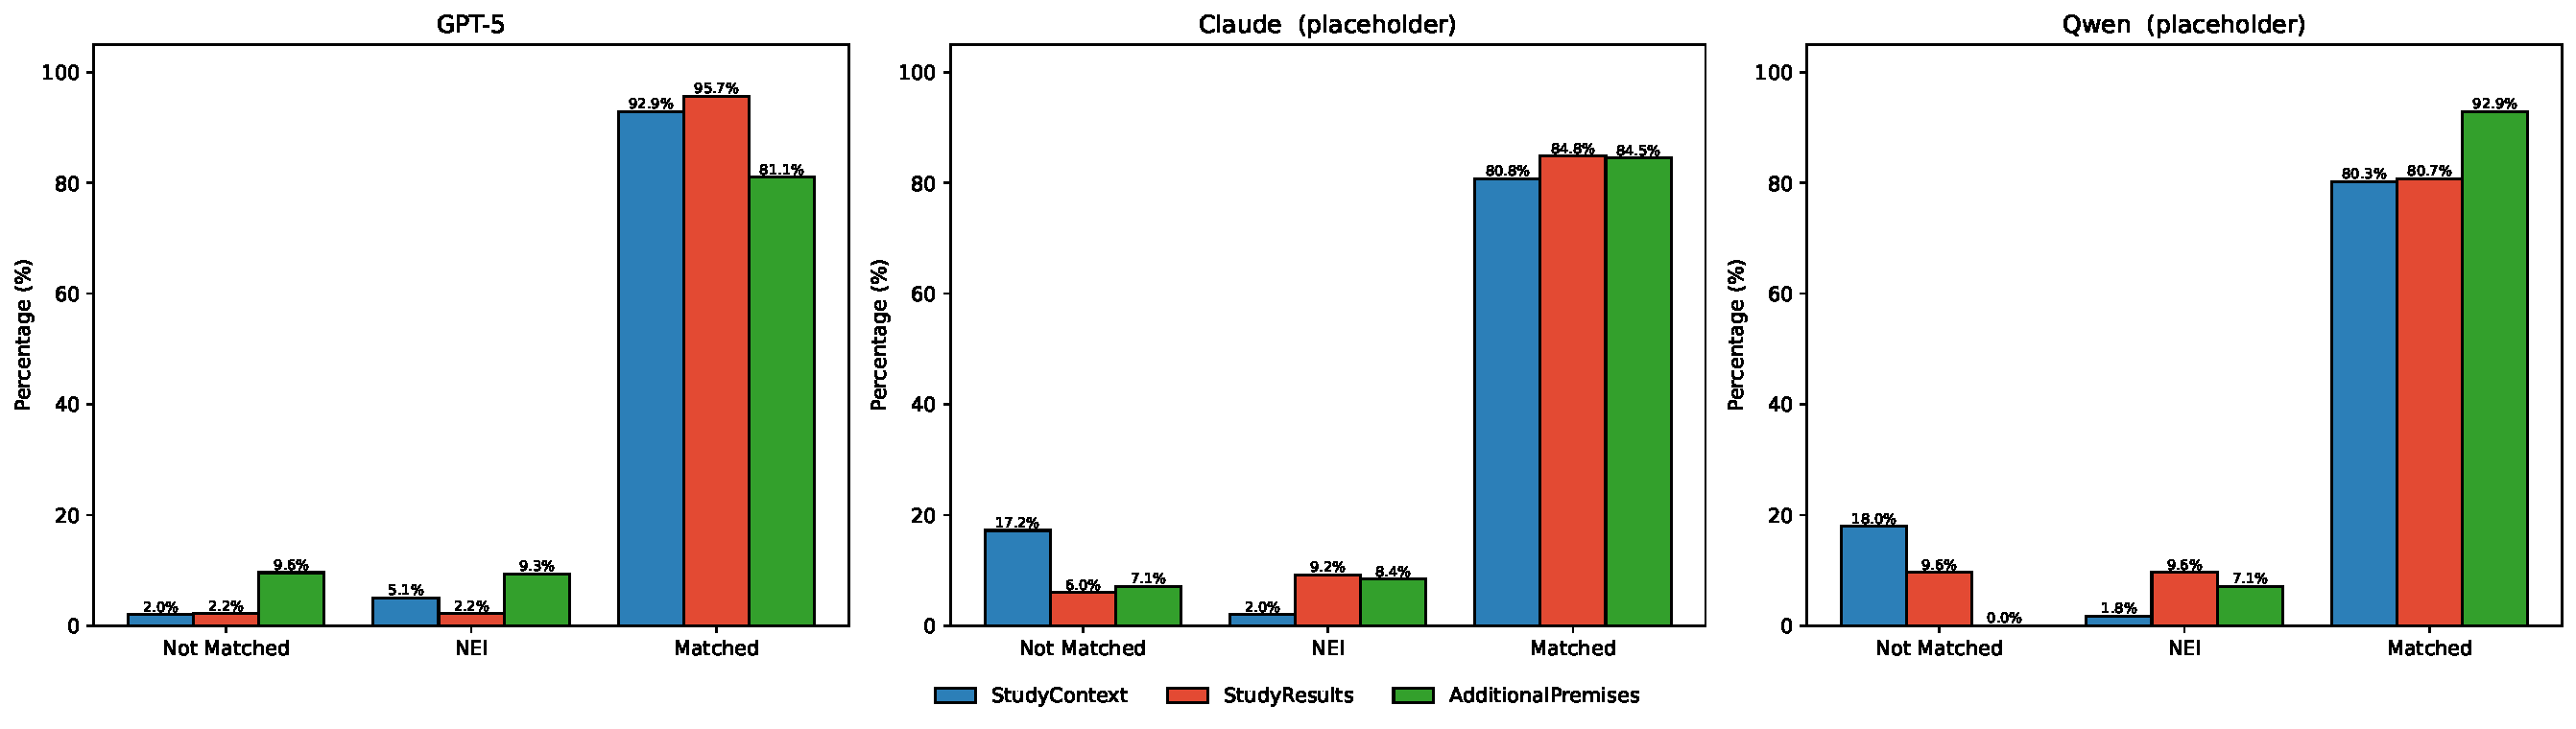
\includegraphics[width=\textwidth]{qa_analysis.pdf}
  \caption{Validation of LLM-generated reasoning graphs against their primary study}
  \label{fig:qa_validation}
\end{figure*}








\section{References}



% Bibliography entries for the entire Anthology, followed by custom entries
%\bibliography{anthology,custom}

% Custom bibliography entries only
\bibliography{custom}

\clearpage
\appendix
\section{Appendix}


This is an appendix.

\begin{figure*}[t]
\small
\centering
\fbox{%
\begin{minipage}{0.97\textwidth}
\begin{flushleft}

\vspace{0.5em}

\ttfamily
You are an expert scientific fact-checker specializing in evaluating whether public claims accurately represent findings from scientific research papers. You have access to the full cited study (provided as a input). Your task is to determine if the claim faithfully reflects the evidence presented in that study.

\vspace{0.5em}

Input

\vspace{0.5em}

\#\#Claim: \\
{[claim]}

\vspace{0.5em}

\#\#Cited Study: \\
{[sutdy]}

\vspace{0.5em}

Instructions

\vspace{0.5em}

1.\ Study Understanding \\
\hspace*{1.5em}Carefully read and summarize the main purpose, methods, and findings of the cited study. \\
\hspace*{1.5em}Identify the key conclusions or outcomes that the authors report.

\vspace{0.5em}

2.\ Claim Interpretation

\vspace{0.5em}

\hspace*{1.5em}Summarize what the claim asserts or implies. \\
\hspace*{1.5em}Identify whether the claim refers to a specific result, a general conclusion, or a causal statement.

\vspace{0.5em}

3.\ Evidence Mapping \\
Locate and quote (or paraphrase) the specific parts of the study that:

\vspace{0.5em}

\hspace*{1.5em}(a) Support the claim, if any. \\
\hspace*{1.5em}(b) Contradict or differ from what the claim asserts. \\
\hspace*{1.5em}(c) Have been distorted or exaggerated by the claim.

\vspace{0.5em}

4.\ Verdict

\vspace{0.5em}

Choose one clear verdict:

\vspace{0.5em}

\hspace*{1.5em}Correct --- The claim correctly represents the cited study. \\
\hspace*{1.5em}Incorrect  --- The claim misrepresents or contradicts the study’s findings. \\
\hspace*{1.5em}Not Enough Information - the study doesn’t provide adequate evidence to support or refute the claim

\vspace{0.5em}

5.\ Reasoning behind verdict \\
Justification and reasoning behind final verdict (3--10 sentences) based on the evidence above.

\vspace{0.5em}

6.\ Output Format \\
\{Justification and reasoning behind final verdict (3--10 sentences) based on the evidence above. \} \\
\{"final\_verdict": "Correct /  Incorrect  / Not Enough Information", \}
\end{flushleft}
\end{minipage}%
}
\caption{Scientific fact-checking prompt used in our study to assess whether a claim faithfully represents the evidence presented in its cited scientific paper.}
\label{fig:factcheck-prompt}
\end{figure*}

\begin{figure*}[t]
\small
\centering
\fbox{%
\begin{minipage}{0.97\textwidth}
\begin{flushleft}

\vspace{0.5em}

\ttfamily
You are a careful annotator. Score the semantic textual similarity (STS) of two text using the rubric the user provides. Reply with valid JSON only.

\vspace{0.5em}

Classify the following pair of arguments by SIMILARITY using this scale:

\vspace{0.5em}

(5)\ Completely equivalent, mean pretty much exactly the same thing, using different words.

\vspace{0.5em}

(4)\ Mostly equivalent, but some unimportant details differ. One argument may be more specific than another or include a relatively unimportant extra fact.

\vspace{0.5em}

(3)\ Roughly equivalent, but some important information differs or is missing. This includes cases where the argument is about the same FACET but the authors have different stances on that facet.

\vspace{0.5em}

(2)\ Not equivalent, but share some details. For example, talking about the same entities but making different arguments (different facets).

\vspace{0.5em}

(1)\ Not equivalent, but are on same topic.

\vspace{0.5em}

(0)\ On a different topic.

\vspace{0.5em}

Text A: \\
\{human\_text\}

\vspace{0.5em}

Textt B: \\
\{llm\_text\}

\vspace{0.5em}

Return only valid JSON in this format:

\vspace{0.5em}

\{\{"sts": <integer from 0 to 5>\}\}

\end{flushleft}
\end{minipage}%
}
\caption{Prompt to calculate STS Score }
\label{fig:sts-prompt}
\end{figure*}



\end{document}
